%---------------------------------------------------------------------------------------------------
% Einf�hrung
%---------------------------------------------------------------------------------------------------
\newpage
%\part{Anfang}
\chapter{Introduction}
\label{cap:Ein}
This bachelor thesis describes the development process of a native android application.
Today life without smart-phone has become unimaginable. It has infiltrated nearly every possible part of humans society. \textit{In the year 2018 two out of three of the people worldwide and 81\% in Germany owns a smart-phone.}
% https://www.wuv.de/digital/weltweite_smartphone_verbreitung_steigt_2018_auf_66_prozent

Applications look like a technical promise of the future. But reminiscending the past is very important to the mankind. Like Elie Wiesel once said:  
"\textit{Without memory, there is no culture. Without memory, there would be no civilization, no society, no future.} - Gefunden auf: https://www.myzitate.de/erinnerungen/Without memory, there is no culture. Without memory, there would be no civilization, no society, no future - Gefunden auf: https://www.myzitate.de/erinnerungen/".

Therefor the Civitas app should help to keep the memory, and store it for upcoming generations. In detail, it is an approach to store historical monument of the roman empire. 

\section{Previous team achivement}

\begin{itemize}
\item User registration
\item User rights plus Admin
\item Filtering
\item Create artefacts
\end{itemize}
\section{Problem statement}

no manual to setup the given project to continue and improve the functionality. on the other hand, use the gained expirience with BaaS to provide a Android and Web app with nice features, such as google map, forget password, mailing service for free. 
Decision to make: spent time to get it running but dont know where to start or start from scratch and provide an app with nice features.

\section{Criteria for success}
everthing is working fine. no bugs around

\subsection{Paragraph A}
hier ist paragraph A
\section{Backendless}
BaaS backend as a service
\section{Java}
Object orientated programming
\begin{figure}[H]
	\centering 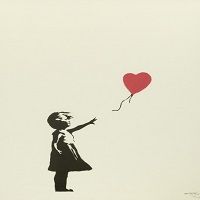
\includegraphics[width=0.8\textwidth]{banksy.jpg}
	\caption[Banksy]{Girl with ballon\footnotemark}
	\label{fig:Banksy}
\end{figure}
\footnotetext{URL: https://www.banksy.org [cited 22 August 2018]}

% Write the Introduction
ich f�hre ein...




 

